\documentclass[uct_visualisation_thesis.tex]{subfiles}

Algorytm UCT, będący usprawnieniem metody MCTS, jest powszechnie stosowanym algorytmem w sztucznej inteligencji. Analizuje on obiecujące ruchy na podstawie generowanego drzewa, równoważąc eksploatację najbardziej zbadanych z eksploracją mniej zbadanych decyzji. Każdemu wierzchołkowi drzewa odpowiada pewien stan rozgrywki, z którego algorytm rozgrywa losowe symulacje, rozszerzając potem drzewo o kolejne możliwe stany. Sposób, w jaki rozrasta się opisywane drzewo, jest kluczowy dla podejmowania przez algorytm obiecujących decyzji. \\

W celu umożliwienia głębszego zrozumienia idei opisywanego zagadnienia postanowiono stworzyć aplikację, która stanowiłaby wygodne narzędzie dla użytkownika zainteresowanego tą tematyką. Pozwalałaby ona na wizualizację drzew stanów algorytmu UCT generowanych podczas rozgrywki w dwie przykładowe gry, co stanowi cel biznesowy projektu.

\section{Harmonogram pracy}
\begin{table}[h!]
	\centering
	\caption{Harmonogram pracy}
	\label{tab:schedule}
	\begin{tabular}{|l|l|}
		\hline
		\textbf{Deadline}   & \textbf{Przygotowane zadania} \\ \hline
		24.10.2019 	& Serializacja \\
		& Algorytm  \\
		& Pierwsza gra \\ \hline
		7.11.2019  	& Podstawowa wizualizacja \\
		& Połączenie algorytmu i gry \\ \hline
		21.11.2019	& Zaawansowana wizualizacja \\
		& Aplikacja okienkowa \\
		& Zapis drzew do pliku graficznego \\ \hline
		5.12.2019 	& Pełna wizualizacja \\
		& Druga gra \\ \hline
		19.12.2019 	& Usprawnienia, poprawki\\ \hline
	\end{tabular}
\end{table}

Czasowy podział pracy nad projektem opisany jest za pomocą harmonogramu w Tabeli \ref{tab:schedule}. Tabela nie opisuje zależności między kolejnymi fazami rozwoju projektu, wyznacza jedynie planowe terminy ich zakończenia. Tworząc tabelę, staraliśmy się rozłożyć pracę regularnie na cały zaplanowany czas tworzenia projektu. Ponadto, ze względu na skomplikowanie modułu odpowiedzialnego za wizualizację, wydzieliliśmy w nim trzy odrębne fazy rozwoju, wymienione poniżej.

\begin{itemize}
	\item Podstawowa wizualizacja -- możliwość wyświetlenia wszystkich wierzchołków drzewa. W podstawowej wizualizacji wygląd wierzchołków jest nieistotny.
	\item Zaawansowana wizualizacja -- podstawowa wizualizacja wzbogacona o możliwość analizowania statystyk poszczególnych wierzchołków. Kolor wierzchołków będzie reprezentował aktualnego gracza.
	\item Pełna wizualizacja -- zaawansowana wizualizacja wzbogacona o możliwość przewijania, przybliżania oraz oddalania podglądu drzewa.
\end{itemize}

\section{Założenia funkcjonalne}
Użytkownik korzystający z naszej aplikacji ma do wyboru jedną z dwóch gier i trzy tryby rozgrywki, wymienione poniżej.

\begin{enumerate}
	\item Gracz versus PC -- użytkownik decyduje o swoich posunięciach i mierzy się on z zaimplementowanym algorytmem.
	\item PC versus PC -- użytkownik jest świadkiem symulacji algorytmu, który rozgrywa partię z samym sobą.
	\item Gracz versus Gracz -- rozgrywka dwóch graczy, bez wizualizacji.
\end{enumerate}
Co więcej, ma on możliwość ustawienia parametrów algorytmu, takich jak liczbę iteracji podczas tworzenia drzewa, czy też maksymalny czas na ruch przeciwnika. Druga opcja, którą dysponuje użytkownik, to możliwość wczytania plików reprezentujących drzewa w formacie zarówno binarnym jak i CSV, a następnie możliwość jego interaktywnej analizy. Może on wyświetlać informacje na temat wybranego węzła, a także przybliżać i oddalać całą wygenerowaną strukturę. Podczas samej rozgrywki, po wykonanym ruchu przeciwnika, gracz może analizować drzewo w sposób opisany powyżej, a także wyeksportować je. Dostępna jest możliwość zapisania go w formatach wymienionych powyżej, a także w formacie rastrowym. Użytkownik może oglądać animację rozrostu drzewa. Powyższe rzeczy dotyczą obu gier w trybach gry z udziałem algorytmu.\\

Diagram przypadków użycia \footnote{Grafika stworzona za pomocą narzędzia na stronie: \url{https://www.lucidchart.com/} -- na zasadzie \textit{free use}}, który ilustruje przedstawione możliwości, znajduje się na Rysunku \ref{rys:usecase}.

\begin{figure}[h!]
	\centering
	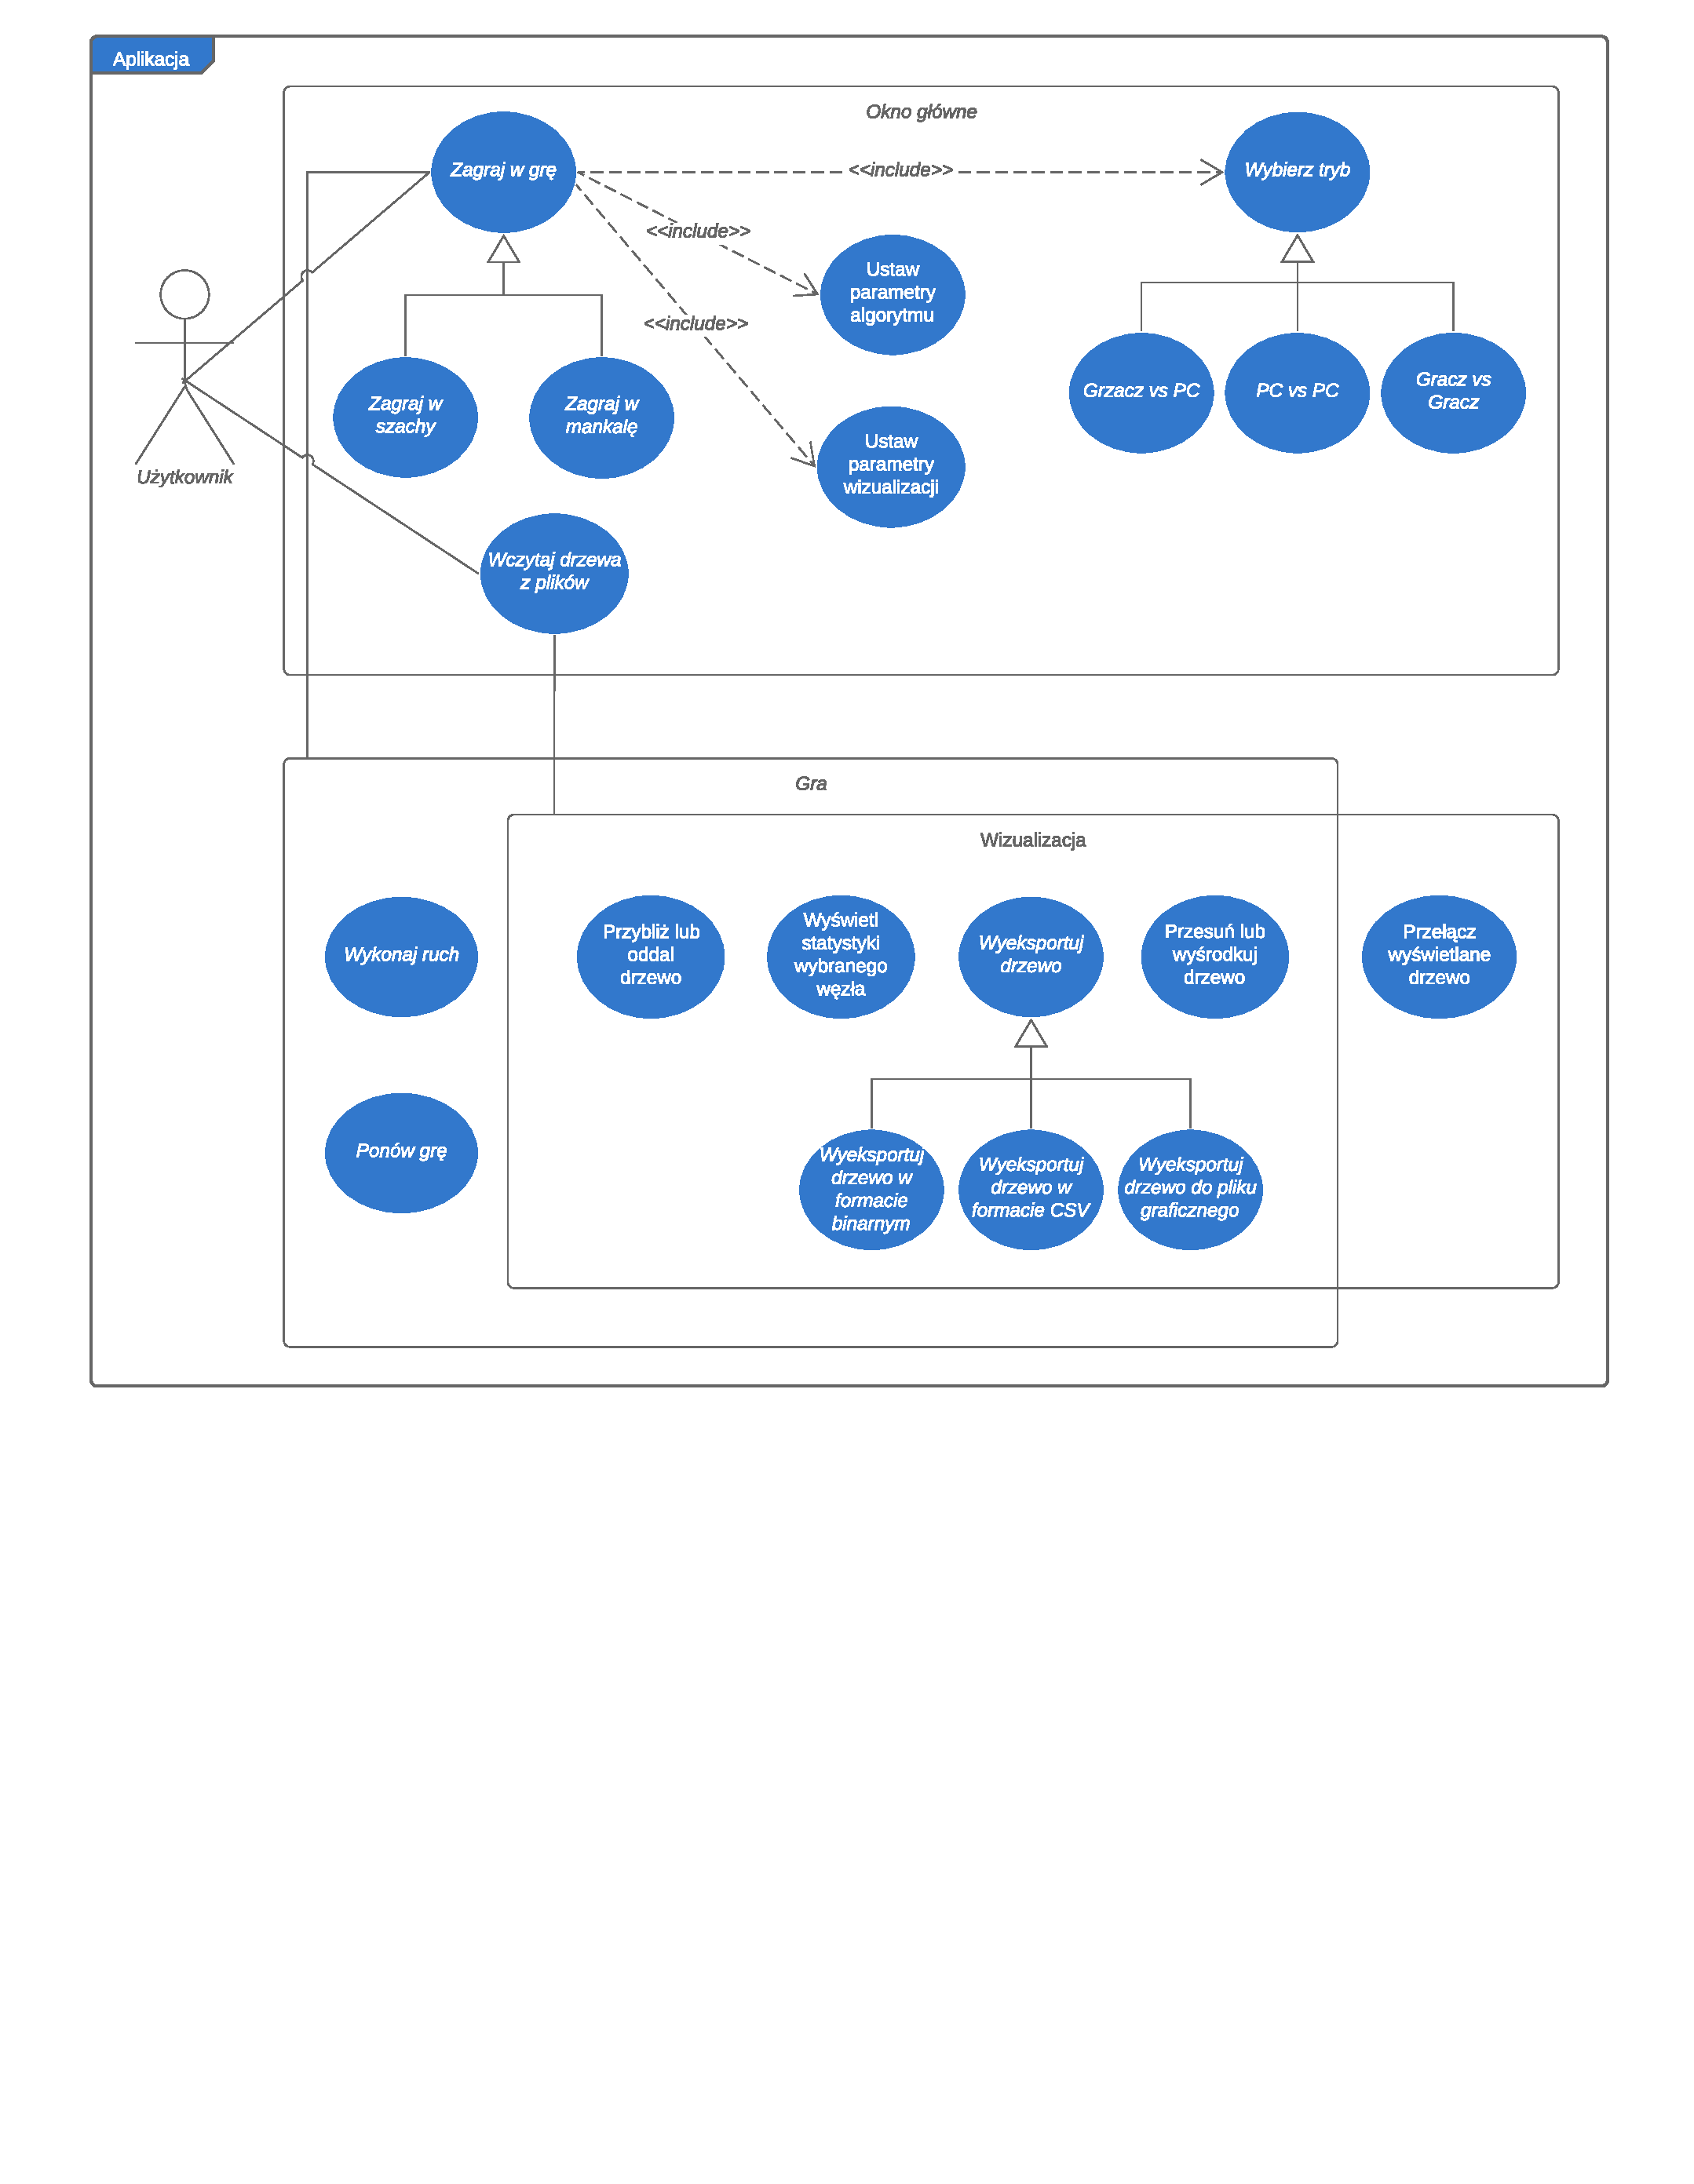
\includegraphics[width=\textwidth, trim={0 6.5cm 0 0},clip]{use-case-simplified-eps}
	\caption{Diagram przypadków użycia}
	\label{rys:usecase}
\end{figure}


\section{Założenia niefunkcjonalne}
Wymagania niefunkcjonalne opisane są w Tabeli \ref{tab:urps}. Zawiera ona opis wymagań sprzętowych aplikacji oraz jej założenia wydajnościowe.

\begin{table}[h!]
	\caption{Analiza założeń niefunkcjonalnych}
	\label{tab:urps}
	\centering
	\begin{tabular}{|l|p{0.7\linewidth}|}
		\hline
		Obszar         & Opis \\ \hline
		Używalność     & Aplikacja działa w jednym oknie wyposażonym w przejrzysty interfejs dla użytkownika. Ponadto, dostarczona jest instrukcja instalacji i obsługi programu.  \\ \hline
		Niezawodność   & Aplikacja działa na komputerze lokalnym i po zainstalowaniu jest dostępna cały czas. Potencjalne błędy nie powinny zamykać aplikacji, a jedynie wyświetlić komunikat dla użytkownika.\\ \hline
		Wydajność      & Aplikacja korzysta głównie z pamięci RAM, procesora i procesora graficznego. Dla drzew do 100 000 wierzchołków wizualizacja nie powinna zajmować więcej niż 3 sekundy, a dla 250 000 --- 5 sekund. Wszystkie obliczenia i wizualizacje są przeprowadzane wewnątrz jednej maszyny.\\ \hline
		Wsparcie       & Aplikacja jest przeznaczona dla komputerów z systemami operacyjnymi Windows oraz Linux opartymi o dystrybucję Debian, na przykład Ubuntu. \\ \hline
	\end{tabular}
\end{table}